\begin{surferPage}{$30$개의 특이점을 갖는 바스의 $6$차식}
	울프 바스가 최다 특이점을 갖는 $6$차식을 만든 후에 그의 두 명의 박사과정 학생은 더 높은 차수의 방정식으로 세계기록을 세웠습니다. 그 후 그는 주어진 차수에 대해 최대 특이점 개수에 대해 고민하기 시작하였습니다. 

Barth의 $65$개의 $A_1^{+-}$(이중 원뿔) 타입의 특이점을 갖는 $6$차식은 $30$개의 뾰족점을 갖는 $6$차식을 만드는데 이용될 수 있습니다. 
    \[P_6 - \alpha \cdot K^3=0,\]
여기서 $P_6$ 는 다른 Barth의 $6$차식처럼 정이십면체와 같은 대칭형태를 갖고 $K$ 는 구의 방정식 입니다. 
    \vspace*{-0.4em}
    \begin{center}
      \begin{tabular}{c@{\ }c@{\ }c@{\ }c}
        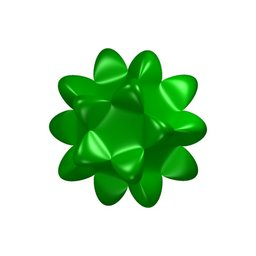
\includegraphics[height=1.2cm]{./../../common/images/barthsextic_30A2}
        &
        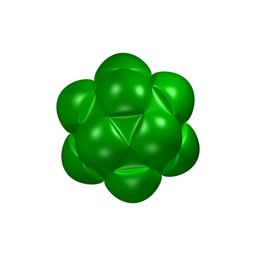
\includegraphics[height=1.2cm]{./../../common/images/barthsextic_30A2_3}
        &
        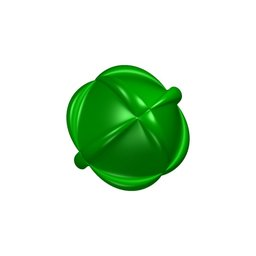
\includegraphics[height=1.2cm]{./../../common/images/barthsextic_30A2_5}
        &
        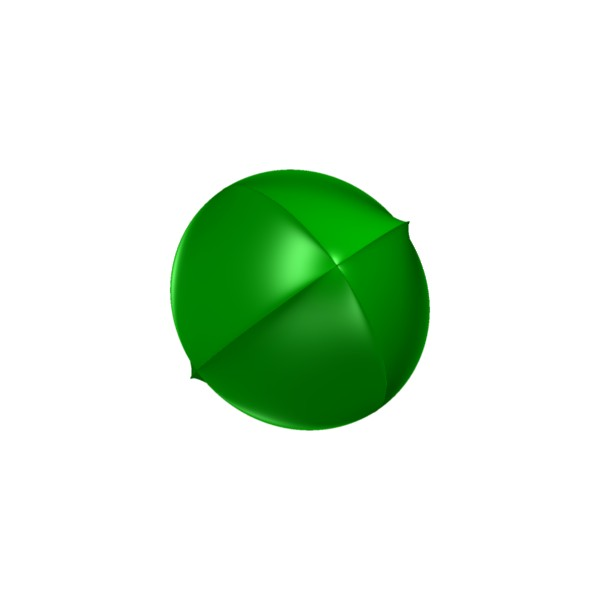
\includegraphics[height=1.2cm]{./../../common/images/barthsextic_30A2_6}
      \end{tabular}
    \end{center}    
    \vspace*{-0.3em}
이것은 현재 $6$차식의 실수 뾰족점의 개수의 세계기록이고 복소수까지 포함하면 $36$개 입니다.
\end{surferPage}
